
\begin{frame}
\frametitle{BreizhCrops Dataset (available by next week!)}

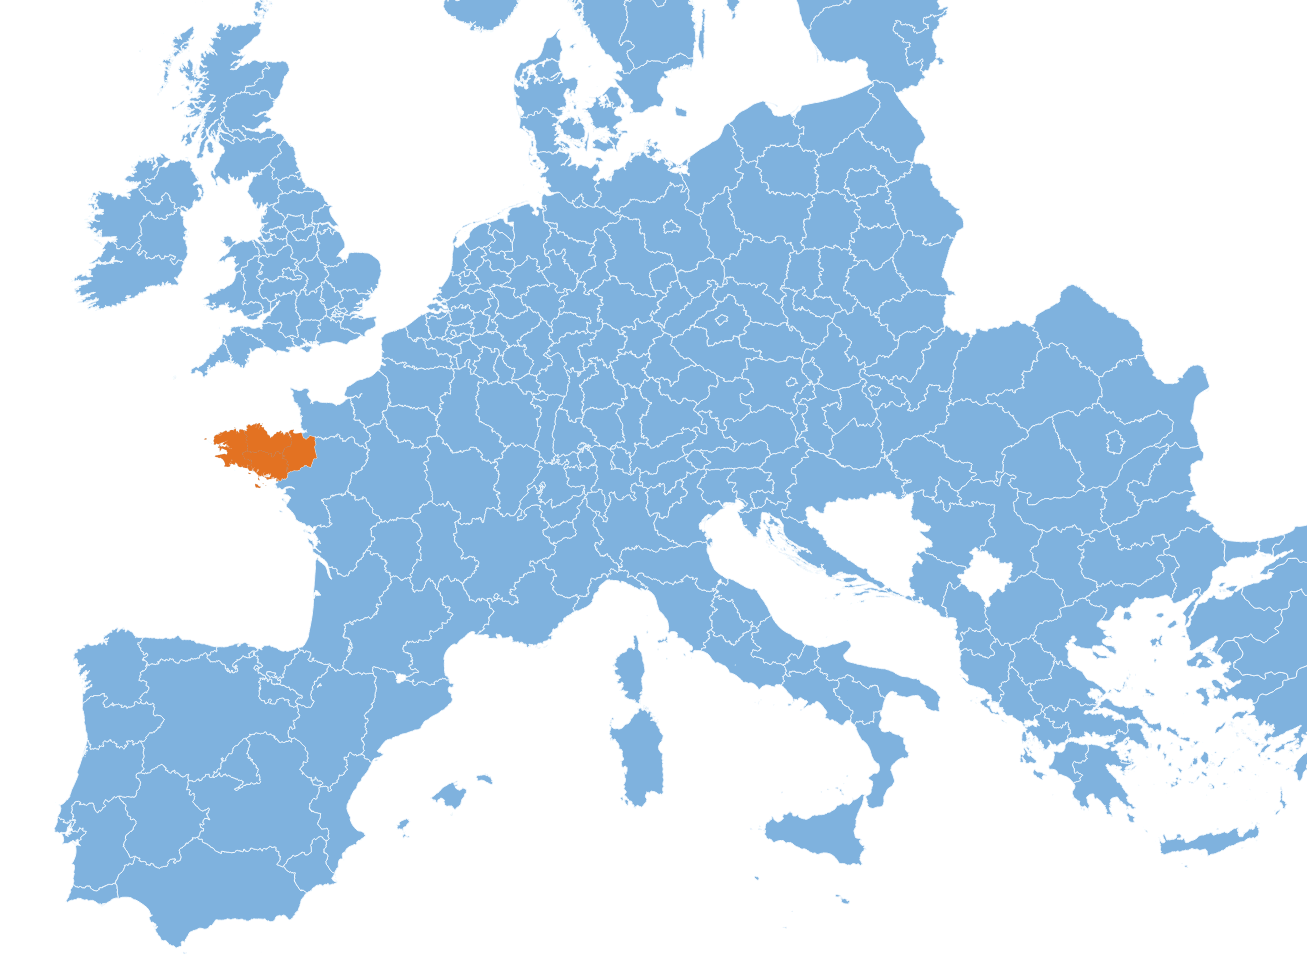
\includegraphics[width=3cm]{images/map/europe}
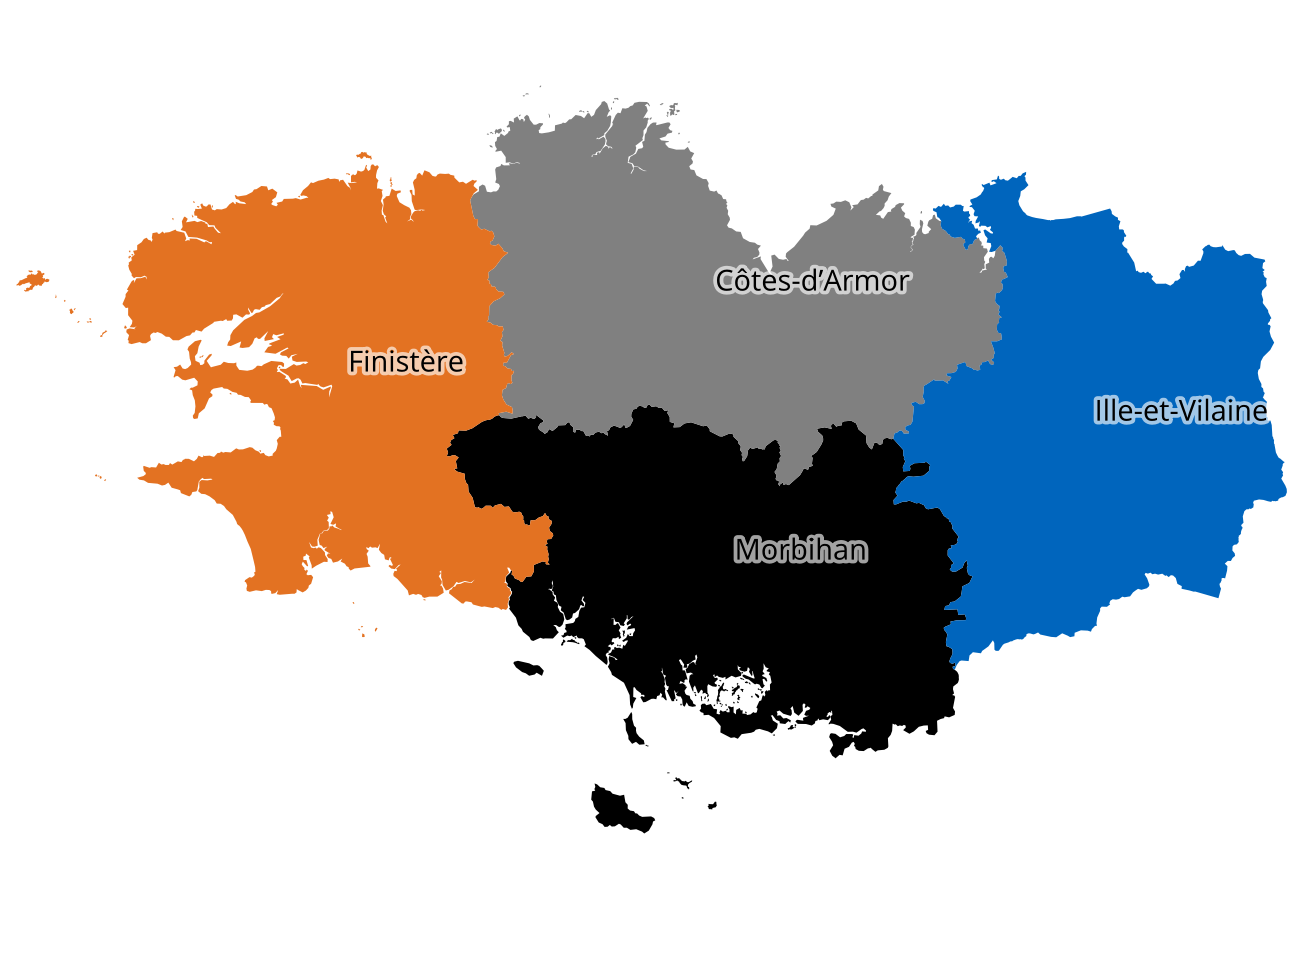
\includegraphics[width=3cm]{images/map/regions}
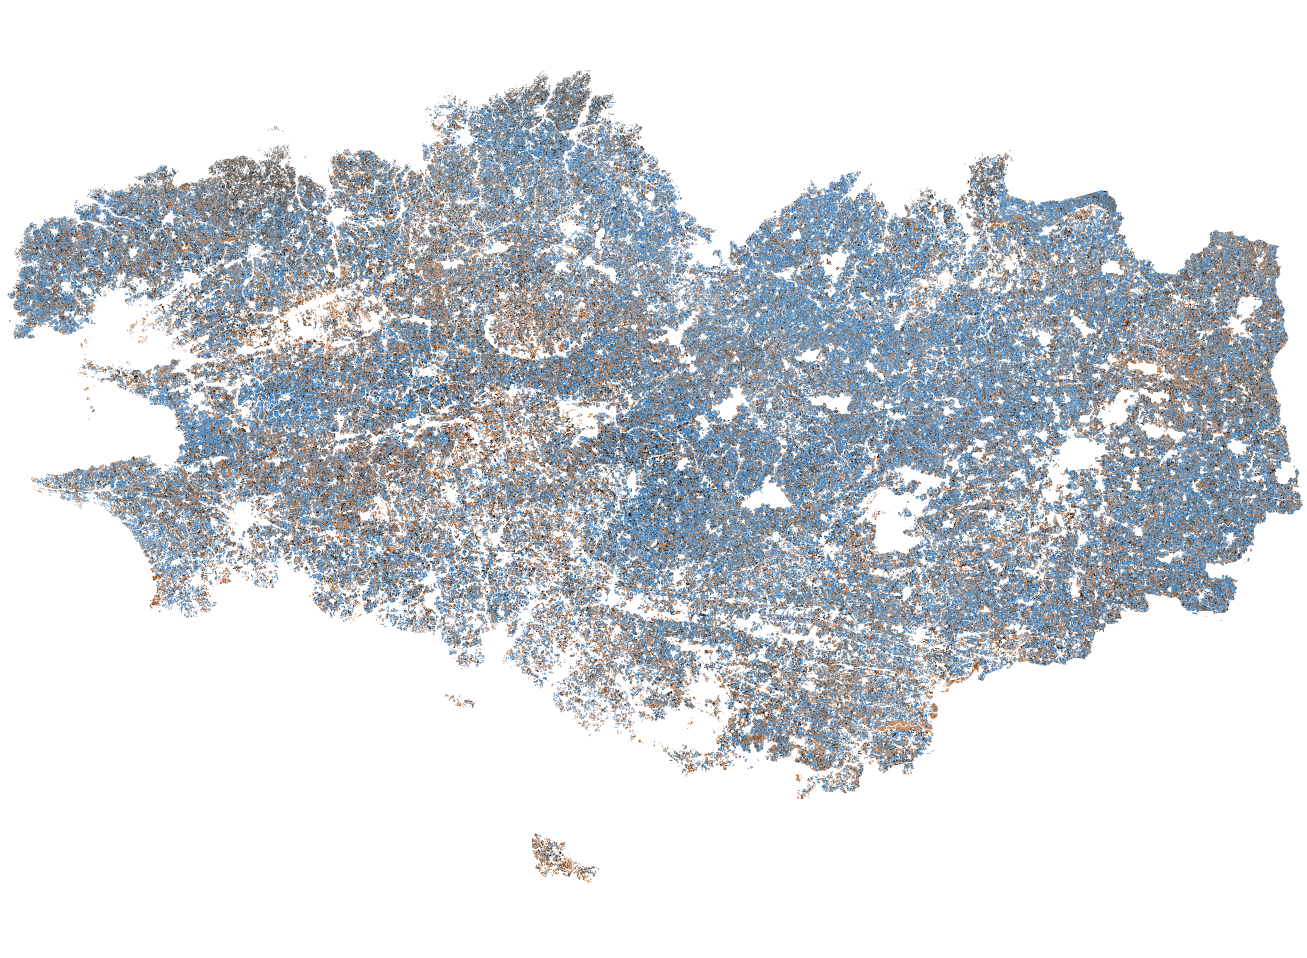
\includegraphics[width=3cm]{images/map/breizh}
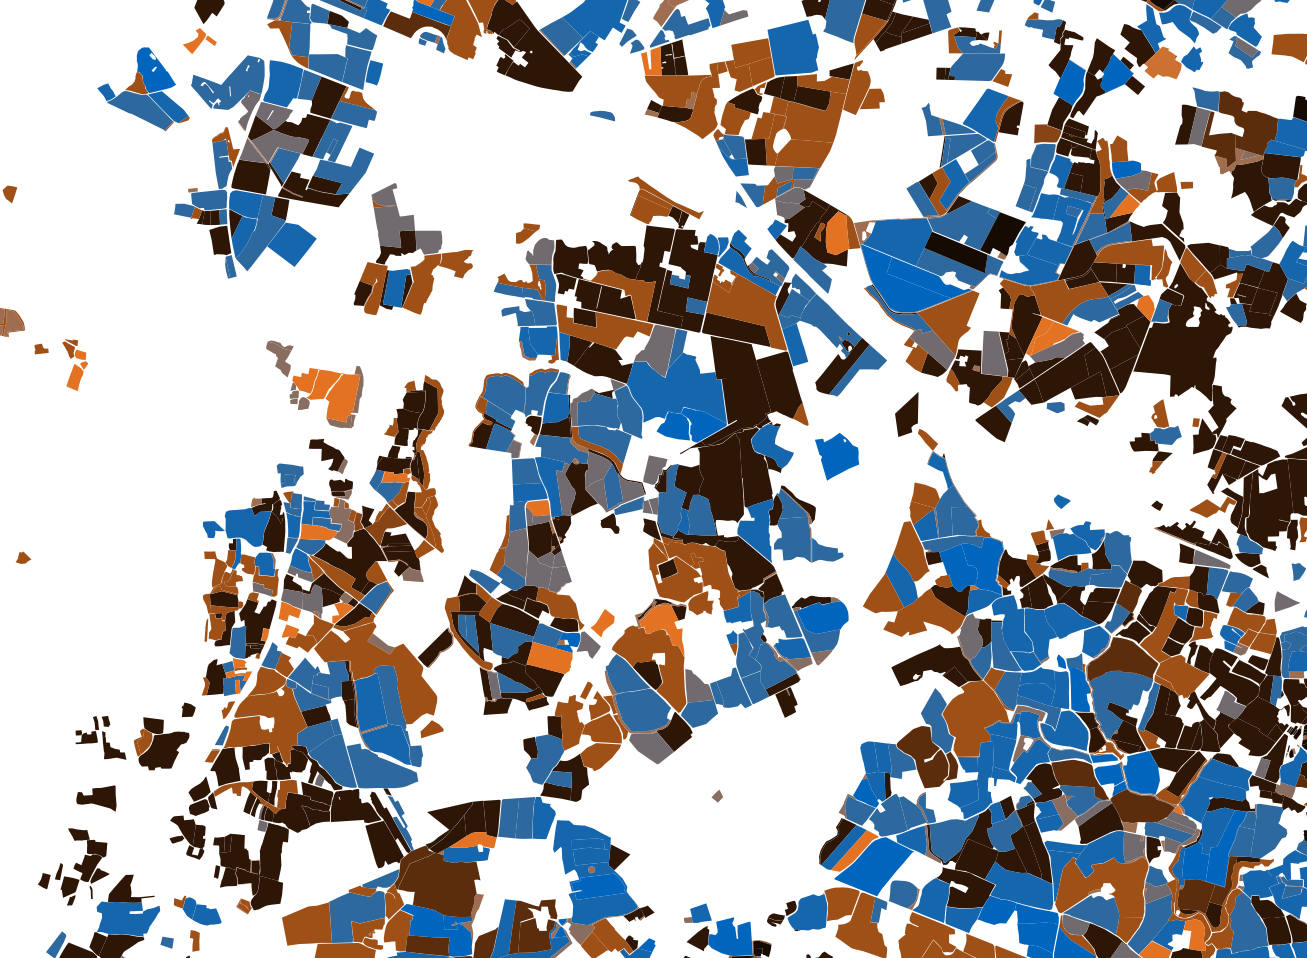
\includegraphics[width=3cm]{images/map/parcels}

\vspace{1em}

%\tikzsetnextfilename{example}

\newcommand{\dataexample}[1]{
	
	
	


\begin{tikzpicture}
	
	\tikzstyle{annot} = [font=\tiny\sffamily, text=tumblue]
	\tikzstyle{point} = [thin, tumbluelight, shorten >= .25em, shorten <= .25em]
	
	% from /home/marc/projects/EV2019/images/example/tstop.txt
	\def\tstopv{0.6285714285714286}
	\def\class{winter barley}
	
	\begin{groupplot}[
	group style={
		group name=my plots,
		group size=1 by 1,
		columns=1,
		xlabels at=edge bottom,
		xticklabels at=edge bottom,
		vertical sep=1em,
	},
	date coordinates in=x,
	date ZERO=2017-01-01,
	xmin=2017-01-01,
	xmax=2017-12-31,
	ylabel near ticks,
	ylabel style={font=\sffamily\small, rotate=-90},
	width=\textwidth,
	height=3cm,
	axis x line=bottom,
	axis y line=left,
%	enlarge x limits=0.01,
	xtick={2017-01-01,2017-05-01,2017-08-01,2017-12-01},
	xticklabels={January,April,August,December},
	ymajorgrids,
    ymax=10000
	]
	
\nextgroupplot[thin,
%	smooth=1pt,
no marks,  
ylabel={},
draw opacity=.8,
%		tension=0.001,
legend columns=2,
%y tick label style={rotate=90},
legend style={at={(.5,1)},anchor=south, line width=1pt, fill=tumblue!10}
]

\addplot[b1color] table [x=doa, y=B1, col sep=comma, forget plot] {#1};
\addplot[b9color] table [x=doa, y=B9, col sep=comma, forget plot] {#1};
\addplot[b10color] table [x=doa, y=B10, col sep=comma] {#1};

\addplot[b11color] table [x=doa, y=B11, col sep=comma, forget plot] {#1};
\addplot[b12color] table [x=doa, y=B12, col sep=comma] {#1};

\addplot[b5color] table [x=doa, y=B5, col sep=comma, forget plot] {#1};
\addplot[b6color] table [x=doa, y=B6, col sep=comma, forget plot] {#1};
\addplot[b7color] table [x=doa, y=B7, col sep=comma, forget plot] {#1};
\addplot[b8color] table [x=doa, y=B8, col sep=comma, forget plot] {#1};
\addplot[b8Acolor] table [x=doa, y=B8A, col sep=comma] {#1};

\addplot[b2color] table [x=doa, y=B2, col sep=comma, forget plot] {#1};
\addplot[b3color] table [x=doa, y=B3, col sep=comma, forget plot] {#1};
\addplot[b4color] table [x=doa, y=B4, col sep=comma] {#1};
	
%	\draw [red, very thick, ->] ([xshift=5em]plt.north west) -- ([xshift=5em]plt.south west) node [midway, rotate=90, fill=white, yshift=2pt] {faster} ;
%	\node(glab) at (10em,0.5) {ground (signal)};
	
%	\sample{images/example/3685593.csv}
%	
%	\sample{images/example/6053223.csv}
%	\draw[fill=white, draw=none, opacity=.5] (axis cs:\tstopv,0) rectangle (axis cs:1,1.1);
	
%	\node[annot](cllab) at (axis cs:.2,1.3) {clouds (noise)};
%	\draw[point] (cllab) -- (axis cs:.13,.7);
%	\draw[point] (cllab) -- (axis cs:.25,.7);
%	\draw[point] (cllab) -- (axis cs:.53,1);
%	\draw[point] (cllab) -- (axis cs:.45,.85);
%	
%	\node[annot](glab) at (axis cs:.8,1.3) {ground (signal)};
%	\draw[point] (glab) -- (axis cs:.38,.3);
%	\draw[point] (glab) -- (axis cs:.21,.3);
%	\draw[point] (glab) -- (axis cs:.7,.3);
%	
%	\draw (axis cs:\tstopv,0) -- (axis cs:\tstopv,1) node[above]{$\tstop$};
%	
%	
%	
%	\legend{3 atmospheric, 2 short-wave infrared, 5 near infrared, 3 visible bands}
%	
		\end{groupplot}
	
	\end{tikzpicture}
	
}
\begin{columns}
	\column{.5\textwidth}
	
	\textbf{corn grain and silage}
	\dataexample{images/breizhcrops/example/6139251.csv}
	
	\column{.5\textwidth}
	
	\textbf{temporary meadows}
	\dataexample{images/breizhcrops/example/3685593.csv}
	
\end{columns}

\vspace{1em}

\Large
580k samples of Time Series $\M{X}$ and labels $\V{y}$. \Large \url{https://github.com/TUM-LMF/BreizhCrops}

\end{frame}


\begin{frame}
	\frametitle{Challenges and Impact}
	
	\Large
	
	\begin{columns}[t]
	
	\column{.5\textwidth}
	
	\visible<1->{
		\textbf{Impact}
		\vspace{1em}
		
		\begin{description}[itemsep=.5em]
		\item large scale \textbf{real-world dataset}
		\item effectively \textbf{unlimited data} (spatially and temporally)
		\item \textbf{assessing generalization} over large regions
		\item potential for further \textbf{vegetation characteristics} (drought indicator, early classification, crop yield)
		\end{description}
	}
	
	\column{.5\textwidth}
	
	\visible<2->{
	\textbf{Challenges}
	\vspace{1em}
	
	\begin{description}[itemsep=.5em]
		\item \textbf{Imbalanced} class \textbf{labels}
		\item Classes with \textbf{similar characteristics}
		\item Non-Gaussian noise induced by \textbf{clouds}
		\item \textbf{Regional} \textbf{variations} in the class distributions
		\item \textbf{Spatial} \textbf{autocorrelation}
		\item \textbf{Irregular} temporal \textbf{sampling} distance
		\item \textbf{Variable} \textbf{sequence} length
	\end{description}
}
	

	\end{columns}
	
\end{frame}


\begin{frame}
\frametitle{Multi-Layer RNN baseline}

\newcommand{\confmat}[3]{

\begin{tikzpicture}

  \def\vmax{#3}
  \def\dataindex{#2}
  
%
%  \pgfplotsset{every axis label/.append style={font=\footnotesize},tick pos=right, ylabel near ticks}
%  
%  \pgfplotsset{
%    axis line style={%
%      opacity=0 
%    }   
%  }

  \begin{groupplot}[
  	group style={
  		group size=2 by 1,
  		xlabels at=edge bottom,
  		ylabels at=edge left,
  		xticklabels at=edge bottom,
  		vertical sep=35pt,
  		group name=seq_len_plot
  	},
  	axis line style={draw=none},
  	title style={yshift=.75em,},
    width=6cm,
    height=6cm,
    enlargelimits=false,
    xtick=data,
%     ymin=1,
    xtick distance=1,
    ytick distance=1,
    colormap={example}{%
		color=(tumwhite)%color=(tumbluelight)
%		color=(tumivory)
%		color=(tumorange)
		color=(tumblue)%color=(tumbluelight)
%		color=(tumblack)
	},
    ytick=data,
    ytick align=outside,
    xtick align=outside,
%    tick style={draw=none},
    ytick pos = left,  
    tick label style = {font=\tiny\sansmath\sffamily},
    %xticklabel = {xshift=-0.75cm}
    yticklabel pos=left,
    %yticklabel near ticks,
    xlabel={\normalsize predicted},
    xlabel style={yshift=1em},
    ylabel style={yshift=-3em},
    x label style={at={(axis description cs:0.5,1)},anchor=south},
    y label style={at={(axis description cs:-0.1,.5)},anchor=south},
    ylabel={\normalsize ground truth},
%     ylabel near ticks,
%    xticklabels={},
  ]
  \nextgroupplot[
%      yticklabels={
%%      	{sugar beet},
%%      	{summer oat},
%%      	{meadow},
%%      	{rape},
%%      	%{vegetable},
%%      	{hop},
%%      	{winter spelt},
%%      	{winter triticale},
%%      	{beans},
%%      	{peas},
%%      	{potato},
%%      	{soybeans},
%%      	{asparagus},
%%      	{winter wheat},
%%      	{winter barley},
%%      	{winter rye},
%%      	{summer barley},
%%      	{maize}
%      },
%      xticklabels={
%%      	{sug.},
%%      	{s. oat},
%%      	{mead.},
%%      	{rape},
%%      	%{vegetable},
%%      	{hop},
%%      	{w. spelt},
%%      	{w. trit.},
%%      	{beans},
%%      	{peas},
%%      	{potato},
%%      	{soyb.},
%%      	{asp.},
%%      	{w. wheat},
%%      	{w. barley},
%%      	{w. rye},
%%      	{s. barley},
%%      	{maize}
%      },
     %colorbar style={title={\precisionrecall}, xshift=0cm, font=\footnotesize},
     colorbar right,
     colorbar style={
        	title={}, 
        	font=\footnotesize,
        	%at={(0,1)},
        	anchor=north west,
        	width=8pt,
        	ticklabel pos=right,
        	ticklabel style={xshift=2em},
%        	label style={yshift=-1em},
        	rounded corners=1pt
     },
  ]
  
    \addplot[
      matrix plot,
%      draw=tumwhite,
%       nodes near coords=\coordindex,
%       nodes near coords align={center},
%       nodes near coords style={font=\scriptsize},
        shader=faceted,
        faceted color=tumgraylight!20,
%       shader=faceted interp,
      mesh/cols=13,
      empty line=scanline,
      point meta=explicit,
      point meta min=0,
      point meta max=\vmax,
    ] table[meta index=\dataindex] {#1};
%   \nextgroupplot[
%       title=2017,
%       %colorbar style={title={\precisionrecall}, xshift=0cm, font=\footnotesize},
%       colorbar right,
%       colorbar style={
%       	title={a}, 
%       	font=\footnotesize,
%       	%at={(0,1)},
%       	anchor=north west,
%       	width=8pt,
%       	ticklabel pos=right,
%       	ticklabel style={xshift=1em},
%       	label style={yshift=1em},
%       	rounded corners=1pt
%       },
%       yticklabels={},
%     xticklabels={
%           	{sug.},
%           	{s. oat},
%           	{mead.},
%           	{rape},
%           	%{vegetable},
%           	{hop},
%           	{w. spelt},
%           	{w. trit.},
%           	{beans},
%           	{peas},
%           	{potato},
%           	{soyb.},
%           	{asp.},
%           	{w. wheat},
%           	{w. barley},
%           	{w. rye},
%           	{s. barley},
%           	{maize}
%     },
%       ]
%    
%    \addplot[
%    matrix plot,
%%    draw=tumwhite,
%    ,   
%    %       nodes near coords=\coordindex,
%    %       nodes near coords align={center},
%    %       nodes near coords style={font=\scriptsize},
%    shader=faceted,
%    faceted color=tumgraylight,
%    %       shader=faceted interp,
%    mesh/cols=17,
%    empty line=scanline,
%    point meta=explicit,
%    point meta min=0,
%    point meta max=\vmax,
%    ] table[meta index=\dataindex] {images/confmat/formatted_grucm2017.csv};
    
  \end{groupplot}
\end{tikzpicture}
}

\begin{columns}
	
	\column{.5\textwidth}
	\textbf{Precision}
	
	\confmat{images/data/BreizhCrops_rnn/npy/confmat_flat.csv}{3}{1}
	
	\column{.5\textwidth}
	\textbf{Recall}
	
	\confmat{images/data/BreizhCrops_rnn/npy/confmat_flat.csv}{4}{1}
	
\end{columns}

\end{frame}

\begin{frame}
\frametitle{Transformer baseline}

\newcommand{\confmat}[3]{

\begin{tikzpicture}

  \def\vmax{#3}
  \def\dataindex{#2}
  
%
%  \pgfplotsset{every axis label/.append style={font=\footnotesize},tick pos=right, ylabel near ticks}
%  
%  \pgfplotsset{
%    axis line style={%
%      opacity=0 
%    }   
%  }

  \begin{groupplot}[
  	group style={
  		group size=2 by 1,
  		xlabels at=edge bottom,
  		ylabels at=edge left,
  		xticklabels at=edge bottom,
  		vertical sep=35pt,
  		group name=seq_len_plot
  	},
  	axis line style={draw=none},
  	title style={yshift=.75em,},
    width=6cm,
    height=6cm,
    enlargelimits=false,
    xtick=data,
%     ymin=1,
    xtick distance=1,
    ytick distance=1,
    colormap={example}{%
		color=(tumwhite)%color=(tumbluelight)
%		color=(tumivory)
%		color=(tumorange)
		color=(tumblue)%color=(tumbluelight)
%		color=(tumblack)
	},
    ytick=data,
    ytick align=outside,
    xtick align=outside,
%    tick style={draw=none},
    ytick pos = left,  
    tick label style = {font=\tiny\sansmath\sffamily},
    %xticklabel = {xshift=-0.75cm}
    yticklabel pos=left,
    %yticklabel near ticks,
    xlabel={\normalsize predicted},
    xlabel style={yshift=1em},
    ylabel style={yshift=-3em},
    x label style={at={(axis description cs:0.5,1)},anchor=south},
    y label style={at={(axis description cs:-0.1,.5)},anchor=south},
    ylabel={\normalsize ground truth},
%     ylabel near ticks,
%    xticklabels={},
  ]
  \nextgroupplot[
%      yticklabels={
%%      	{sugar beet},
%%      	{summer oat},
%%      	{meadow},
%%      	{rape},
%%      	%{vegetable},
%%      	{hop},
%%      	{winter spelt},
%%      	{winter triticale},
%%      	{beans},
%%      	{peas},
%%      	{potato},
%%      	{soybeans},
%%      	{asparagus},
%%      	{winter wheat},
%%      	{winter barley},
%%      	{winter rye},
%%      	{summer barley},
%%      	{maize}
%      },
%      xticklabels={
%%      	{sug.},
%%      	{s. oat},
%%      	{mead.},
%%      	{rape},
%%      	%{vegetable},
%%      	{hop},
%%      	{w. spelt},
%%      	{w. trit.},
%%      	{beans},
%%      	{peas},
%%      	{potato},
%%      	{soyb.},
%%      	{asp.},
%%      	{w. wheat},
%%      	{w. barley},
%%      	{w. rye},
%%      	{s. barley},
%%      	{maize}
%      },
     %colorbar style={title={\precisionrecall}, xshift=0cm, font=\footnotesize},
     colorbar right,
     colorbar style={
        	title={}, 
        	font=\footnotesize,
        	%at={(0,1)},
        	anchor=north west,
        	width=8pt,
        	ticklabel pos=right,
        	ticklabel style={xshift=2em},
%        	label style={yshift=-1em},
        	rounded corners=1pt
     },
  ]
  
    \addplot[
      matrix plot,
%      draw=tumwhite,
%       nodes near coords=\coordindex,
%       nodes near coords align={center},
%       nodes near coords style={font=\scriptsize},
        shader=faceted,
        faceted color=tumgraylight!20,
%       shader=faceted interp,
      mesh/cols=13,
      empty line=scanline,
      point meta=explicit,
      point meta min=0,
      point meta max=\vmax,
    ] table[meta index=\dataindex] {#1};
%   \nextgroupplot[
%       title=2017,
%       %colorbar style={title={\precisionrecall}, xshift=0cm, font=\footnotesize},
%       colorbar right,
%       colorbar style={
%       	title={a}, 
%       	font=\footnotesize,
%       	%at={(0,1)},
%       	anchor=north west,
%       	width=8pt,
%       	ticklabel pos=right,
%       	ticklabel style={xshift=1em},
%       	label style={yshift=1em},
%       	rounded corners=1pt
%       },
%       yticklabels={},
%     xticklabels={
%           	{sug.},
%           	{s. oat},
%           	{mead.},
%           	{rape},
%           	%{vegetable},
%           	{hop},
%           	{w. spelt},
%           	{w. trit.},
%           	{beans},
%           	{peas},
%           	{potato},
%           	{soyb.},
%           	{asp.},
%           	{w. wheat},
%           	{w. barley},
%           	{w. rye},
%           	{s. barley},
%           	{maize}
%     },
%       ]
%    
%    \addplot[
%    matrix plot,
%%    draw=tumwhite,
%    ,   
%    %       nodes near coords=\coordindex,
%    %       nodes near coords align={center},
%    %       nodes near coords style={font=\scriptsize},
%    shader=faceted,
%    faceted color=tumgraylight,
%    %       shader=faceted interp,
%    mesh/cols=17,
%    empty line=scanline,
%    point meta=explicit,
%    point meta min=0,
%    point meta max=\vmax,
%    ] table[meta index=\dataindex] {images/confmat/formatted_grucm2017.csv};
    
  \end{groupplot}
\end{tikzpicture}
}

\begin{columns}
	
	\column{.5\textwidth}
	\confmat{images/data/BreizhCrops_transformer/npy/confmat_flat.csv}{3}{1}
	
	\column{.5\textwidth}
	\confmat{images/data/BreizhCrops_transformer/npy/confmat_flat.csv}{4}{1}
	
\end{columns}

\end{frame}


\begin{frame}
\frametitle{Going Big...}

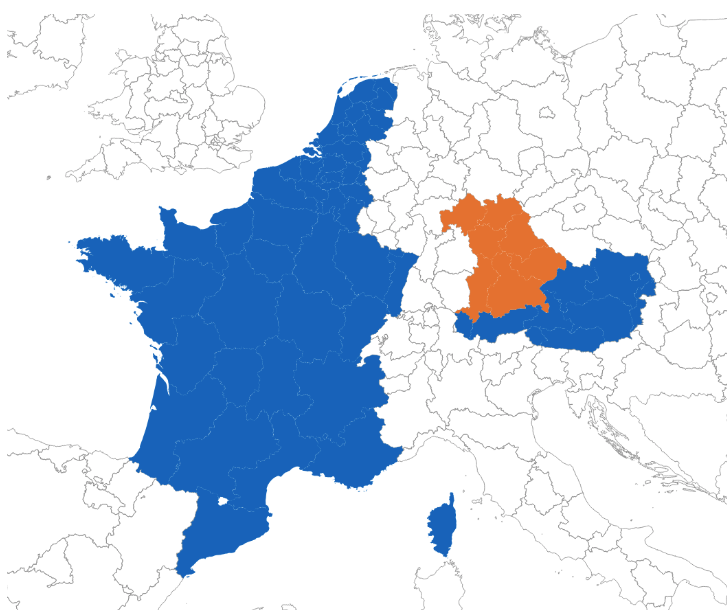
\includegraphics[width=5cm]{images/EuroCrops}
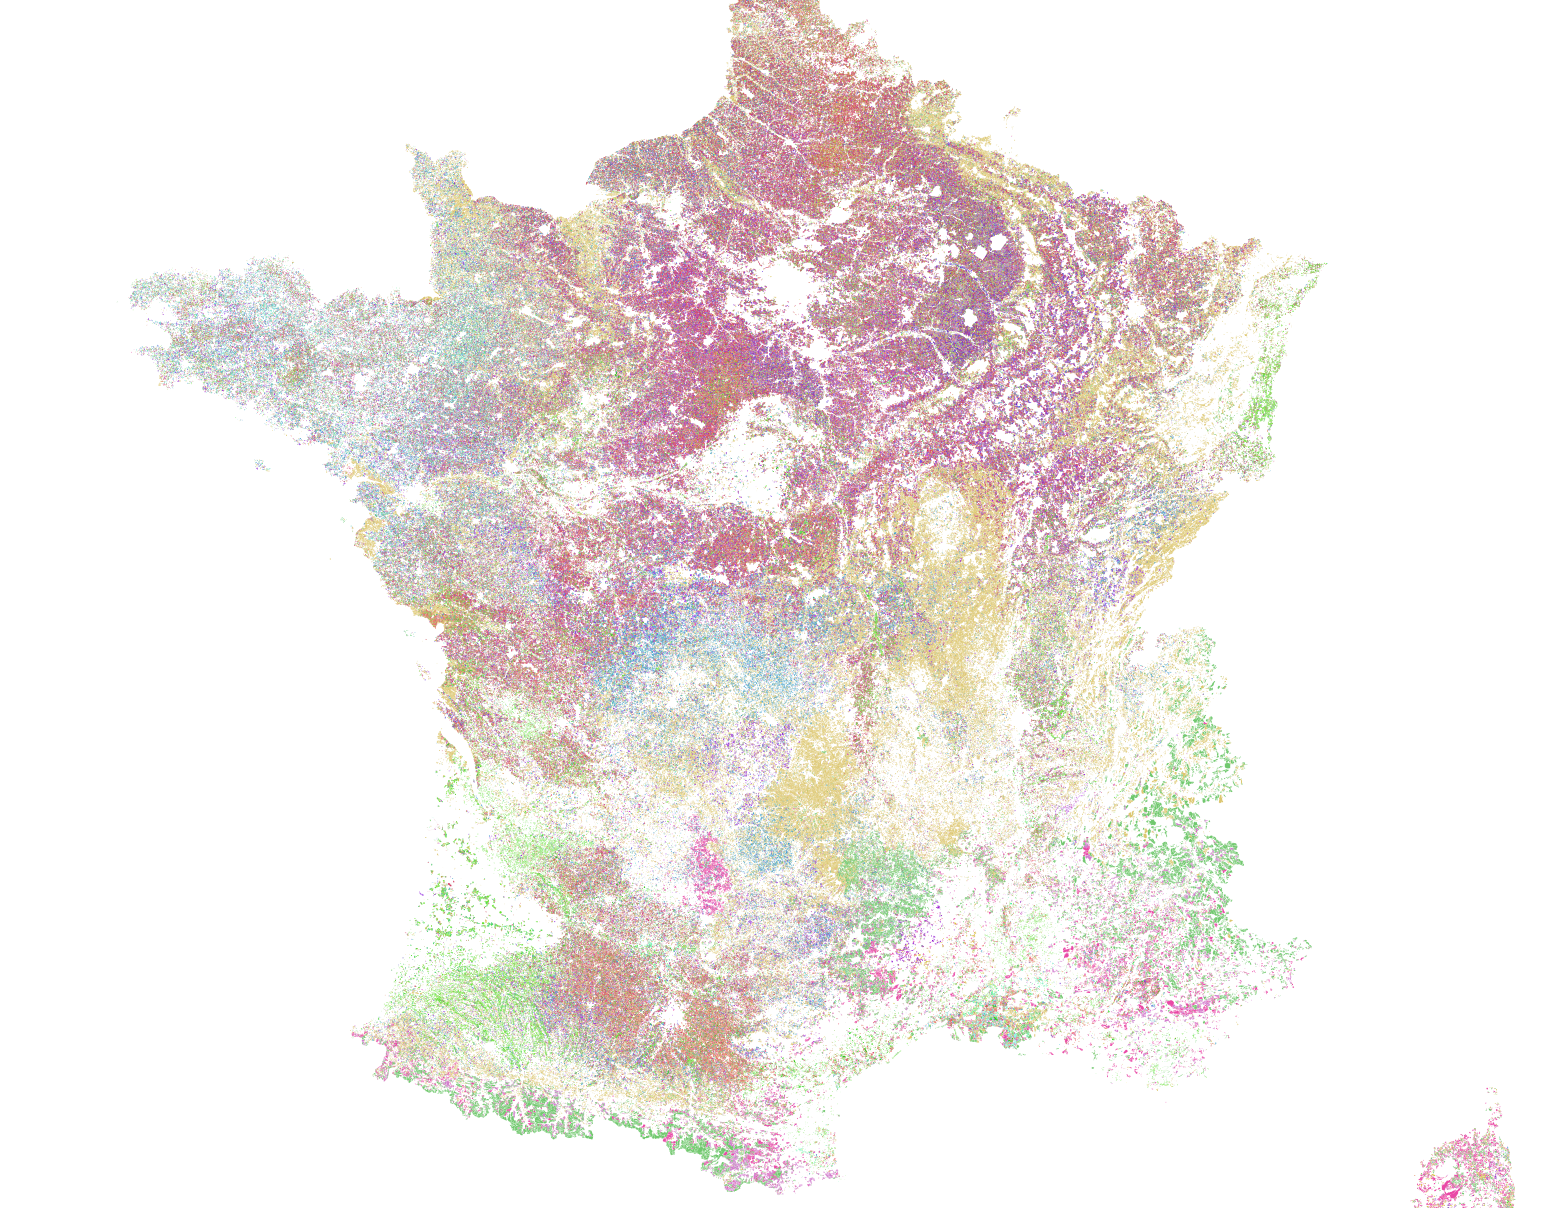
\includegraphics[width=5cm]{images/France}
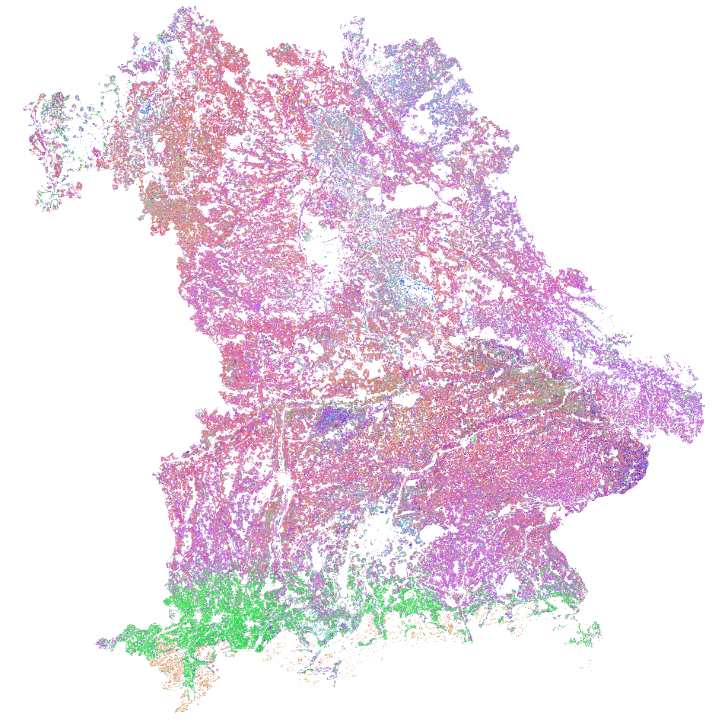
\includegraphics[width=4cm]{images/Bavaria}

\end{frame}

\begin{frame}
\frametitle{Supported by Google Research Credits}


\includegraphics[width=.3\textwidth]{images/google_research_credits}

\includegraphics[width=.3\textwidth]{images/google}

\includegraphics[width=.2\textwidth]{images/earth-engine-logo}
%
\includegraphics[width=3cm]{images/250px-Google-Cloud-Storage-Logo}
%
\includegraphics[width=3cm]{images/Google_Compute_Engine_logo}
%
\includegraphics[width=3cm]{images/google_cloud_sql}


\end{frame}
